\documentclass[a4paper]{article}

\def\npart {UD BMEG 671}
\def\nterm {Module 2}
\def\nyear {2026}
\def\nlecturer {Islam and Zurakowski; DiStefano; current modeling guidance}
\def\ncourse {Module 2: Nonlinear Systems, Stability, and Dosing Workflows}
\def\ncoursehead {Nonlinear Systems}
\def\nauthor {NanFangHong}

\RequirePackage{etex}
\makeatletter
\ifx \npart \undefined
  \def\npart{PK/PD Notes}
\fi
\ifx \nterm \undefined
  \def\nterm{Reading notes}
\fi
\ifx \nyear \undefined
  \def\nyear{\the\year}
\fi
\ifx \nlecturer \undefined
  \def\nlecturer{the source literature}
\fi
\ifx \nauthor \undefined
  \def\nauthor{NanFangHong}
\fi
\ifx \ncourse \undefined
  \def\ncourse{Pharmacology Reading Note}
\fi
\ifx \ncoursehead \undefined
  \def\ncoursehead{\ncourse}
\fi

\author{Based on \nlecturer \\\small Notes taken by \nauthor}
\date{\nterm\ \nyear}
\title{\npart\ --- \ncourse}

\usepackage{amsfonts}
\usepackage{amsmath}
\usepackage{amssymb}
\usepackage{amsthm}
\usepackage{booktabs}
\usepackage{caption}
\usepackage{enumitem}
\usepackage{fancyhdr}
\usepackage{fontspec}
\usepackage{graphicx}
\usepackage{iftex}
\usepackage{mathtools}
\usepackage{microtype}
\usepackage{siunitx}
\usepackage{tabularx}
\usepackage{tikz}
\usepackage{xcolor}
\usepackage{xurl}
\usepackage{xeCJK}

\IfFontExistsTF{Latin Modern Roman}{
  \setmainfont[Ligatures=NoCommon]{Latin Modern Roman}
}{}

\IfFontExistsTF{Noto Serif CJK SC}{
  \setCJKmainfont{Noto Serif CJK SC}
}{
  \IfFontExistsTF{Songti SC}{
    \setCJKmainfont{Songti SC}
  }{
    \IfFontExistsTF{PingFang SC}{
      \setCJKmainfont{PingFang SC}
    }{}
  }
}

\usepackage[hidelinks,unicode,breaklinks=true]{hyperref}
\hypersetup{
  pdfauthor={\nauthor},
  pdfsubject={\npart\ - \ncourse},
  pdftitle={\npart\ - \ncourse},
  pdfkeywords={PK PD pharmacology reading notes \ncourse}
}

\pagestyle{fancyplain}
\lhead{\emph{\nouppercase{\leftmark}}}
\rhead{
  \ifnum\thepage=1
  \else
    \npart\ \ncoursehead
  \fi}

\theoremstyle{definition}
\newtheorem*{aim}{Aim}
\newtheorem*{assumption}{Assumption}
\newtheorem*{defi}{Definition}
\newtheorem*{eg}{Example}
\newtheorem*{notation}{Notation}
\newtheorem*{question}{Question}
\newtheorem*{remark}{Remark}
\newtheorem*{warning}{Warning}

\theoremstyle{plain}
\newtheorem{nthm}{Theorem}[section]
\newtheorem{nprop}[nthm]{Proposition}

\renewcommand{\labelitemi}{--}
\renewcommand{\labelitemii}{$\circ$}
\renewcommand{\labelenumi}{(\roman{*})}

\let\stdsection\section
\renewcommand\section{\newpage\stdsection}

\newcommand{\dd}{\mathop{}\!\mathrm{d}}
\newcommand{\Emax}{E_{\max}}
\newcommand{\pksym}[1]{\ifmmode\text{\textit{#1}}\else\textit{#1}\fi}
\newcommand{\pklab}[1]{\mathrm{#1}}
\newcommand{\ECfifty}{\pksym{EC}_{50}}
\newcommand{\term}[1]{\emph{#1}}
\makeatother

\title{UD BMEG 671 Module 2 --- Nonlinear Systems,\\ Stability, and Dosing Workflows}
\author{Based on BMEG/ELEG 471/671 lectures\\\small DiStefano and current modeling guidance\\\small Notes taken by NanFangHong}
\usetikzlibrary{arrows.meta,positioning,calc,decorations.pathreplacing,fit,shapes.geometric}
\emergencystretch=4em
\sloppy
\captionsetup{width=0.9\textwidth, justification=raggedright, singlelinecheck=false}
\lhead{\emph{\npart}}
\rhead{\ncoursehead}

\DeclareMathOperator{\rank}{rank}
\DeclareMathOperator{\tr}{tr}
\DeclareMathOperator{\diag}{diag}
\DeclareMathOperator{\eig}{eig}
\DeclareMathOperator{\sgn}{sgn}
\newcommand{\R}{\mathbb{R}}
\newcommand{\ddt}{\frac{\dd}{\dd t}}
\newcommand{\vect}[1]{\boldsymbol{#1}}
\newcommand{\mat}[1]{\mathbf{#1}}
\newcommand{\J}{\mat J}
\newcommand{\A}{\mat A}
\newcommand{\B}{\mat B}
\newcommand{\C}{\mat C}
\newcommand{\Obs}{\mathcal O}
\newcommand{\Ctrb}{\mathcal C}
\newcommand{\Rpos}{\R_{\ge 0}}
\newcommand{\Rzero}{\mathcal R_0}
\newcommand{\given}{\,|\,}
\newcommand{\Prob}{\mathbb{P}}
\newcommand{\Ex}{\mathbb{E}}
\newcommand{\PK}{\ensuremath{\pksym{PK}}}
\newcommand{\PD}{\ensuremath{\pksym{PD}}}
\newcommand{\PKPD}{\ensuremath{\pksym{PK}/\pksym{PD}}}
\newcommand{\QSP}{\ensuremath{\pksym{QSP}}}
\newcommand{\PBPK}{\ensuremath{\pksym{PBPK}}}
\newcommand{\MIDD}{\ensuremath{\pksym{MIDD}}}
\newcommand{\SBML}{\ensuremath{\pksym{SBML}}}
\newcommand{\MATLAB}{\ensuremath{\pksym{MATLAB}}}
\newcommand{\SimBio}{\ensuremath{\pksym{SimBiology}}}
\newcommand{\SIR}{\ensuremath{\pksym{SIR}}}
\newcommand{\AUC}{\ensuremath{\pksym{AUC}}}
\newcommand{\CL}{\ensuremath{\pksym{CL}}}
\newcommand{\code}[1]{\texttt{#1}}
\newcommand{\Vmax}{V_{\max}}
\newcommand{\Km}{K_m}

\definecolor{bmegblue}{HTML}{114B7A}
\definecolor{bmegteal}{HTML}{178F88}
\definecolor{bmeggreen}{HTML}{4E8F4A}
\definecolor{bmegpurple}{HTML}{6651A6}
\definecolor{bmegred}{HTML}{B94444}
\definecolor{bmegorange}{HTML}{C77A2B}
\definecolor{bmeglight}{HTML}{F3F6F7}
\tikzset{
  comp/.style={draw=bmegblue!75, fill=bmeglight, rounded corners=2pt, align=center, inner sep=5pt, minimum width=24mm, minimum height=9mm},
  state/.style={draw=bmegpurple!75, fill=white, rounded corners=2pt, align=center, inner sep=5pt, minimum width=23mm, minimum height=9mm},
  flow/.style={-{Stealth[length=2.2mm]}, thick, draw=bmegblue!90},
  loss/.style={-{Stealth[length=2.2mm]}, thick, draw=bmegred!90},
  dashedflow/.style={-{Stealth[length=2.2mm]}, thick, dashed, draw=bmegpurple!85},
  info/.style={font=\footnotesize, align=center}
}

\begin{document}
\maketitle
{\small
  \noindent\textbf{Reading motive}\\
  这是 UD BMEG/ELEG 471/671 在 2025 年 9 月 8 日到 9 月 26 日这一组课的学习笔记。前一篇笔记把 compartment, state, input, output, mass balance, linear simulation, verification and validation 搭成了建模语法；这一篇接着问一个更深的问题：当模型变成 nonlinear ODE 以后，我们怎样判断它能不能被观测、能不能被输入驱动、会不会回到稳态、会不会越过生物上不允许的边界、什么时候会振荡，以及怎样把这些判断落实到 \MATLAB{} 和 \SimBio{} workflow 里。\par\hfill[course note]

  \vspace{5pt}
  \noindent\textbf{Reader}\\
  假设读者已经读过第一篇 BMEG 671 note，知道一室/二室模型、step input、impulse dose、matrix form 和 basic ODE simulation。这里不会假设读者已经懂 dynamical systems；相反，每个定理都从它在 biomedical modeling 里的用途讲起。\par\hfill[from modeling grammar to model behavior]

  \vspace{5pt}
  \noindent\textbf{Update}\\
  课程主线来自本地 lecture notes、transcripts、\MATLAB{} live scripts 和 \SimBio{} projects \cite{bmeg671Lectures3to10Slides2025,bmeg671TranscriptsSep08to262025,bmeg671MatlabNonlinearStability2025,bmeg671SimBiologyProjects2025}. 我也把它放在 2026 年仍然重要的语境里：\MIDD{} 要求模型围绕 question of interest、model evaluation、documentation and decision consequence 组织证据；\SimBio{}、\SBML{} 和 ASME V\&V 40 则提醒我们，图、方程、代码、单位和可信度是同一个工作流的不同面 \cite{ichM15Midd2026,fdaMiddProgram2026,mathworksSimBiologyTutorials2026,sbmlLevel3Version2Release2,asmeVV402018}.
}

\tableofcontents

\section{The Second Spine}

\subsection{From writing equations to understanding behavior}

The first part of the course taught the grammar:
\[
  \text{compartment diagram}\longrightarrow
  \dot{\vect q}=f(\vect q,\vect u,\vect\theta,t)\longrightarrow
  \vect y=g(\vect q,\vect\theta,t).
\]
This second part asks what the equations imply. Once a model is written, the central questions change:
\begin{itemize}[leftmargin=2em]
  \item Can the hidden states be inferred from the measured outputs?
  \item Can the input actually move the system in the directions we care about?
  \item Near a biological operating point, can a nonlinear system be approximated by a linear one?
  \item Which steady states are stable, unstable, or biologically irrelevant?
  \item Does the model preserve nonnegativity of concentrations, cell counts, and viral loads?
  \item Are oscillations real attracting cycles or merely initial-condition-dependent closed orbits?
  \item When a dose is given repeatedly or piecewise, should it be encoded as a reaction, an input, a dose object, or a segmented simulation?
\end{itemize}

The lectures answer these questions in a deliberately practical order. They start with \SimBio{} because a graphical model builder forces us to name species, reactions, parameters, units, and dose objects. They then return to matrix and nonlinear analysis because no graphical tool can replace the mathematical questions of observability, controllability, stationary points, stability, and invariance.

\subsection{A map of the lectures}

The course materials from September 8--26 form one arc:
\begin{center}
\begin{tabularx}{0.92\textwidth}{@{}lX@{}}
Sep 8 & \SimBio{}, \SIR{}, linearization, and matrix review\\
Sep 10 & observability and controllability\\
Sep 12 & mass action, Michaelis--Menten, Hill functions, logistic growth\\
Sep 17 & stationary points, \SIR{} stability, Lyapunov methods\\
Sep 19 & Lyapunov first method and positive invariance\\
Sep 22 & limit cycles, fox-rabbit dynamics, parameter-range stability\\
Sep 24 & virus-host model, vaccine dosing, \MATLAB{} and \SimBio{} dose workflow\\
Sep 26 & exercises: stable equilibria, positive invariance, and interpretation
\end{tabularx}
\end{center}
The details look diverse, but the hidden object is always the same: a vector field. Given
\[
  \dot{\vect x}=f(\vect x,\vect u,\vect\theta,t),
\]
we want to know what the arrows in state space do.

\subsection{Why nonlinear behavior enters so early}

Linear models are the cleanest possible classroom entrance. But real biomedical systems become nonlinear almost immediately:
\begin{itemize}[leftmargin=2em]
  \item infection terms often use products such as \(\beta SI\);
  \item enzymatic elimination saturates like \(\Vmax q/(\Km+q)\);
  \item receptor occupancy and signaling often have sigmoidal Hill functions;
  \item immune expansion, tumor growth, and cell populations are bounded by resource limits;
  \item dose schedules are discontinuous in time;
  \item biological state variables must remain nonnegative.
\end{itemize}
The course therefore does not treat nonlinearity as advanced ornament. It is the normal state of biomedical modeling.

\section{SimBiology as Equation Grammar}

\subsection{What a graphical model builder is really checking}

\SimBio{} appears in the lectures as software, but mathematically it is a grammar checker. To build a model, the user must decide:
\begin{center}
compartments, species, reactions, parameters, units, doses, and outputs.
\end{center}
This is not clerical work. These choices define the ODE. A reaction diagram that looks reasonable can still be wrong if the rate law has the wrong units, if a dose targets the wrong species, or if a hidden state is never connected to measurement.

The Sep 8 lecture uses \SIR{} to show how a familiar epidemic story becomes a model. In a basic closed \SIR{} system:
\[
  \begin{aligned}
  \dot S &= -\beta SI,\\
  \dot I &= \beta SI-aI,\\
  \dot R &= aI.
  \end{aligned}
\]
The reaction \(S+I\to 2I\) is second order in the state variables. If \(S\) and \(I\) are amounts or concentrations, \(\beta\) must carry reciprocal amount per time units. If \(S\) and \(I\) are fractions of a normalized population, the unit bookkeeping changes. This is why the transcript repeatedly warns that dimension and unit are not the same thing \cite{bmeg671TranscriptsSep08to262025}.

\subsection{The same diagram can hide different equations}

A graphical arrow is visually simple. A rate law is not. Consider a reaction \(A+B\to C\). Under mass action,
\[
  R=k[A][B].
\]
The corresponding ODE contribution is
\[
  \dot A=-R,\qquad \dot B=-R,\qquad \dot C=R.
\]
But if the reaction is enzyme limited, transporter mediated, or receptor mediated, the same visual arrow may be better represented by Michaelis--Menten or Hill kinetics. The diagram tells the topology; the rate law tells the dynamics.

This is one reason \SBML{} and \SimBio{} matter beyond convenience. They encourage explicit representation of species, compartments, reactions, parameters, and units, so the model can be inspected, exchanged, and tested \cite{sbmlLevel3Version2Release2,mathworksSimBiologyTutorials2026}. In a regulatory or collaborative setting, that explicitness is part of credibility.

\subsection{When to use equation-first modeling}

Some course examples are awkward to draw as standard reactions. The vaccine model, for instance, uses an antigen-like input \(u(t)\) and a memory-like state \(b(t)\):
\[
  \begin{aligned}
  \dot a &= -d_a a+u(t),\\
  \dot b &= \lambda-d_b b+eab.
  \end{aligned}
\]
The term \(eab\) is an interaction term. It can be represented in a reaction network, but the equation is more transparent. The practical rule is:
\begin{center}
\fbox{\parbox{0.87\textwidth}{\centering If the diagram clarifies conservation and topology, draw it. If the equation clarifies the mechanism and input schedule, write the equation first. Then make the two agree.}}
\end{center}

\section{Linearization}

\subsection{Why linearize a nonlinear model}

Linearization is the bridge between nonlinear biology and linear systems tools. Suppose
\[
  \dot{\vect x}=f(\vect x,\vect u)
\]
and we care about behavior near an operating point \((\bar{\vect x},\bar{\vect u})\). First-order Taylor expansion gives
\[
  \dot{\vect x}
  \approx
  f(\bar{\vect x},\bar{\vect u})
  +\left.\frac{\partial f}{\partial \vect x}\right|_{(\bar{\vect x},\bar{\vect u})}
   (\vect x-\bar{\vect x})
  +\left.\frac{\partial f}{\partial \vect u}\right|_{(\bar{\vect x},\bar{\vect u})}
   (\vect u-\bar{\vect u}).
\]
If the operating point is a stationary point under the baseline input, then
\[
  f(\bar{\vect x},\bar{\vect u})=0,
\]
and the perturbation variables \(\delta\vect x=\vect x-\bar{\vect x}\), \(\delta\vect u=\vect u-\bar{\vect u}\) satisfy approximately
\[
  \delta\dot{\vect x}=\A\delta\vect x+\B\delta\vect u,
  \qquad
  \A=\left.\frac{\partial f}{\partial \vect x}\right|_{(\bar{\vect x},\bar{\vect u})},
  \quad
  \B=\left.\frac{\partial f}{\partial \vect u}\right|_{(\bar{\vect x},\bar{\vect u})}.
\]
This is why a nonlinear system can still be studied with eigenvalues, observability matrices, and controllability matrices, provided the question is local.

\subsection{The Jacobian is the local arrow map}

For \(\dot{\vect x}=f(\vect x)\), the Jacobian is
\[
  \J(\vect x)=
  \begin{bmatrix}
  \frac{\partial f_1}{\partial x_1} & \cdots & \frac{\partial f_1}{\partial x_n}\\
  \vdots & \ddots & \vdots\\
  \frac{\partial f_n}{\partial x_1} & \cdots & \frac{\partial f_n}{\partial x_n}
  \end{bmatrix}.
\]
Each entry asks: if I slightly increase state \(x_j\), how does the derivative of state \(x_i\) change? In biomedical language, it is a local sensitivity of flux direction to state perturbation.

For the basic \SIR{} model,
\[
  f(S,I,R)=
  \begin{bmatrix}
  -\beta SI\\
  \beta SI-aI\\
  aI
  \end{bmatrix},
\]
so
\[
  \J(S,I,R)=
  \begin{bmatrix}
  -\beta I & -\beta S & 0\\
  \beta I & \beta S-a & 0\\
  0 & a & 0
  \end{bmatrix}.
\]
At a disease-free state with \(I=0\), the sign of \(\beta S-a\) tells whether a small infected perturbation grows or decays. That one derivative is already the seed of the reproduction-threshold argument.

\subsection{Linearization is not the model}

The lecture's warning is subtle: linearization is local. It says what the nonlinear system does near the selected point. It does not guarantee global behavior. A tumor-growth model can be locally stable near carrying capacity and still biologically impossible if it permits negative tumor mass elsewhere. A viral model can have a locally stable infection equilibrium and still fail if its parameter range violates known biology. Local stability is a useful lens, not a license to stop thinking.

\section{Observability}

\subsection{The question observability answers}

Observability asks whether hidden states can be reconstructed from outputs. In biomedical modeling this is not optional. We often measure only one or two quantities:
\[
  \text{plasma drug},\quad
  \text{biomarker},\quad
  \text{viral load},\quad
  \text{tumor volume},\quad
  \text{antibody titer}.
\]
The model may contain tissue concentrations, intracellular species, infected-cell counts, or memory states that are never measured directly. Observability asks whether the output time course carries enough information about them.

For a linear time-invariant system
\[
  \dot{\vect x}=\A\vect x+\B\vect u,\qquad \vect y=\C\vect x,
\]
the observability matrix is
\[
  \Obs =
  \begin{bmatrix}
  \C\\
  \C\A\\
  \C\A^2\\
  \vdots\\
  \C\A^{n-1}
  \end{bmatrix}.
\]
The system is observable if
\[
  \rank(\Obs)=n.
\]
The rows \(\C,\C\A,\C\A^2,\ldots\) encode not just what is measured now, but what its derivatives reveal through the dynamics.

\subsection{The four-compartment classroom example}

The Sep 10 lecture uses a four-state example to make the idea concrete. One convenient representation is:
\[
  \A=
  \begin{bmatrix}
  -3&0&0&0\\
  1&-1&0&0\\
  2&0&-1&0\\
  0&1&1&0
  \end{bmatrix},
  \qquad
  \C=\begin{bmatrix}0&0&0&1\end{bmatrix}.
\]
Here the output sees only the fourth state. A diagrammatic version is:
\begin{center}
\resizebox{0.88\textwidth}{!}{%
\begin{tikzpicture}[node distance=26mm]
  \node[state] (x1) {\(x_1\)};
  \node[state, right=of x1] (x2) {\(x_2\)};
  \node[state, below=14mm of x2] (x3) {\(x_3\)};
  \node[state, right=30mm of x2] (x4) {\(x_4=y\)};
  \draw[loss] (x1) -- ++(-18mm,0) node[left,info]{loss};
  \draw[flow] (x1) -- node[above,info]{1} (x2);
  \draw[flow] (x1) -- node[left,info]{2} (x3);
  \draw[loss] (x2) -- ++(0,12mm) node[above,info]{loss};
  \draw[loss] (x3) -- ++(0,-12mm) node[below,info]{loss};
  \draw[flow] (x2) -- node[above,info]{} (x4);
  \draw[flow] (x3) -- node[below,info]{} (x4);
\end{tikzpicture}
}
\end{center}
Computing
\[
  \Obs=
  \begin{bmatrix}
  0&0&0&1\\
  0&1&1&0\\
  3&-1&-1&0\\
  -12&1&1&0
  \end{bmatrix}
\]
shows rank deficiency. Intuitively, \(x_2\) and \(x_3\) enter \(x_4\) symmetrically through a sum, so measuring only \(x_4\) cannot fully separate them.

If we add a second output, for example measuring \(x_2\) as well,
\[
  \C=
  \begin{bmatrix}
  0&1&0&0\\
  0&0&0&1
  \end{bmatrix},
\]
the observability can improve. This is the modeling lesson: if a hidden state is scientifically important but unobservable under the current measurement design, the solution is not algebraic optimism. The solution is a better experiment, an added output, or a simpler model.

\subsection{Observability and identifiability are cousins}

Observability concerns states. Identifiability concerns parameters. They are not the same, but they often fail for the same structural reason: the output does not contain enough distinguishable information. In a two-tissue \PK{} model, two hidden compartments may have exchange rates that are mathematically interchangeable if only total plasma concentration is measured. In a viral model, infected cells and free virions may be hard to separate if only viral load is observed. The course introduces observability before parameter estimation because it forces the right question: what can the data possibly know?

\section{Controllability}

\subsection{The question controllability answers}

Controllability asks whether inputs can move states. In pharmacology, the input is often dose. In systems biology, it may be a perturbation, inhibitor, stimulus, gene knockdown, or feeding protocol. For a linear system,
\[
  \dot{\vect x}=\A\vect x+\B\vect u,
\]
the controllability matrix is
\[
  \Ctrb=
  \begin{bmatrix}
  \B&\A\B&\A^2\B&\cdots&\A^{n-1}\B
  \end{bmatrix}.
\]
The system is controllable if
\[
  \rank(\Ctrb)=n.
\]

The lecture derives this from Taylor expansion of the matrix exponential. With zero initial condition,
\[
  \vect x(t)=\int_0^t e^{\A(t-\tau)}\B\vect u(\tau)\,\dd\tau.
\]
The powers \(\B,\A\B,\A^2\B,\ldots\) are the directions the input can reach directly and indirectly through the system dynamics. If their span does not cover the whole state space, some directions are unreachable.

\subsection{Why pharmacologists should care}

A dose does not control every hidden biological state. Oral dosing controls the gut input. Intravenous infusion controls central exposure. A receptor agonist controls receptor occupancy only through concentration, binding, turnover, and feedback. A vaccine dose controls antigen exposure but not directly memory-cell expansion. Controllability gives language to a familiar problem:
\begin{center}
\fbox{\parbox{0.87\textwidth}{\centering A desired biological state is not necessarily reachable just because we can administer an input.}}
\end{center}

This matters for model-based design. If a target tissue state is not controllable by the proposed dosing route, no optimization algorithm can invent control authority. Conversely, if a model suggests controllability, it tells us which input schedules might be worth testing.

\subsection{Local controllability of nonlinear models}

For nonlinear systems, controllability is more delicate. The course uses the linear rank test as the entry point. Around an operating point,
\[
  \delta\dot{\vect x}=\A\delta\vect x+\B\delta\vect u.
\]
If the linearized system is not controllable, that is a warning. If it is controllable, we gain local evidence, not a global guarantee. Nonlinear systems can have barriers, saturation, safety limits, or positivity constraints that linear approximations ignore.

\section{Kinetic Building Blocks}

\subsection{Mass action}

Mass action is the first mechanistic rate law. For
\[
  A+B\longrightarrow C,
\]
the rate is
\[
  R=k[A][B].
\]
If \(A\) and \(B\) are concentrations, a second-order rate constant has units concentration\(^{-1}\) time\(^{-1}\). The ODE signs are determined by stoichiometry:
\[
  \dot A=-R,\qquad \dot B=-R,\qquad \dot C=R.
\]
For a first-order reaction \(A\to B\), the rate becomes \(R=kA\). For a zero-order input, the rate is constant. In \PK{}, first-order loss and transfer terms are common because they make linear models; in \PD{}, infection, binding, feedback, growth, and enzyme limitation often force products or saturating functions.

\subsection{Michaelis--Menten}

Michaelis--Menten kinetics summarize enzyme-limited conversion:
\[
  E+S \rightleftharpoons ES \longrightarrow E+P.
\]
Under the quasi-steady-state approximation,
\[
  v(S)=\frac{\Vmax S}{\Km+S}.
\]
Two limits matter more than the formula itself:
\[
  S\ll \Km:\quad v(S)\approx \frac{\Vmax}{\Km}S,
  \qquad
  S\gg \Km:\quad v(S)\approx \Vmax.
\]
At low substrate, the system looks first order. At high substrate, it becomes capacity limited. This is why saturable elimination can destroy linear dose proportionality. A doubling of input does not necessarily double exposure if elimination is already near \(\Vmax\).

The \MATLAB{} live scripts use equations such as
\[
  \dot q=\pksym{IR}-\frac{Cq}{K+q}
\]
to compare low-input and high-input regimes \cite{bmeg671MatlabNonlinearStability2025}. When \(\pksym{IR}<C\), a steady state exists:
\[
  q^\ast=\frac{\pksym{IR}\,K}{C-\pksym{IR}}.
\]
As \(\pksym{IR}\) approaches \(C\), the steady state grows sharply. If \(\pksym{IR}\ge C\), the input overwhelms maximal elimination and no finite steady state exists in this simple model. That is the pharmacological meaning of capacity.

\subsection{Hill functions}

Hill functions represent sigmoidal response:
\[
  v(S)=\frac{\Vmax S^n}{K^n+S^n}.
\]
When \(n=1\), this is Michaelis--Menten-shaped. Larger \(n\) creates a sharper transition; smaller effective slopes create a gentler one. The lecture treats Hill functions as empirical \PD{} building blocks. That is the right default. A Hill coefficient can suggest cooperativity, but in fitted biomedical models it often functions as a flexible curve-shape parameter rather than proof of a microscopic mechanism.

\subsection{Logistic growth}

Logistic growth is the minimal bounded-growth model:
\[
  \dot T=\alpha T\left(1-\frac{T}{T_{\max}}\right).
\]
It contains two stationary points:
\[
  T^\ast=0,\qquad T^\ast=T_{\max}.
\]
The derivative of the right-hand side is
\[
  f'(T)=\alpha\left(1-\frac{2T}{T_{\max}}\right).
\]
Thus \(T=0\) is locally unstable when \(\alpha>0\), while \(T=T_{\max}\) is locally stable. The biology is intuitive: a small positive population grows away from extinction, but growth slows and returns toward carrying capacity when near \(T_{\max}\).

\section{Stationary Points}

\subsection{Equilibrium is a model statement, not a moral judgment}

A stationary point \(\vect x^\ast\) satisfies
\[
  f(\vect x^\ast)=0.
\]
It is a state at which the model's instantaneous derivative vanishes. It is not necessarily healthy, desired, or realistic. A disease-free equilibrium, endemic equilibrium, high-tumor equilibrium, and toxic-drug steady state can all be stationary points.

The workflow is:
\begin{enumerate}[leftmargin=2em]
  \item solve \(f(\vect x)=0\);
  \item discard mathematically valid but biologically impossible states, such as negative concentrations;
  \item compute the Jacobian at each remaining point;
  \item analyze eigenvalues or use a Lyapunov argument;
  \item interpret the result in the context of model purpose and parameter ranges.
\end{enumerate}

\subsection{Local stability by eigenvalues}

For
\[
  \dot{\vect x}=f(\vect x),
\]
linearize at \(\vect x^\ast\):
\[
  \delta\dot{\vect x}=\J(\vect x^\ast)\delta\vect x.
\]
If all eigenvalues of \(\J(\vect x^\ast)\) have negative real parts, the stationary point is locally asymptotically stable. If at least one eigenvalue has positive real part, it is unstable. If eigenvalues lie on the imaginary axis or have zero real part, the linear test is inconclusive.

This is the lecture's ``Lyapunov second method'' entry point. In many engineering texts this is called Lyapunov's indirect method. The naming matters less than the warning: the eigenvalue test depends on the first nonzero local term. When the linear term vanishes, the nonlinear terms decide.

\subsection{Two-dimensional shortcut}

For a two-state linearized system with Jacobian
\[
  \J=
  \begin{bmatrix}
  a&b\\c&d
  \end{bmatrix},
\]
the characteristic polynomial is
\[
  \lambda^2-\tr(\J)\lambda+\det(\J)=0.
\]
Local asymptotic stability occurs when
\[
  \tr(\J)<0,\qquad \det(\J)>0.
\]
This is often faster than writing the eigenvalues explicitly, and it is especially useful for epidemic and ecological two-state reductions.

\section{An Endemic SI Model}

\subsection{Model and stationary points}

The Sep 17 lecture studies a birth-death infection model. Let \(S\) be susceptible individuals and \(I\) infected individuals:
\[
  \begin{aligned}
  \dot S &= B-dS-\beta SI,\\
  \dot I &= \beta SI-aI.
  \end{aligned}
\]
Here \(B\) is recruitment into susceptibility, \(d\) is susceptible loss, \(\beta\) is infection transmission, and \(a\) is infected loss or recovery/removal. The stationary points are
\[
  (S^\ast,I^\ast)=\left(\frac{B}{d},0\right)
\]
and, when it is biologically nonnegative,
\[
  (S^\ast,I^\ast)=
  \left(\frac{a}{\beta},\frac{B}{a}-\frac{d}{\beta}\right).
\]
The second equilibrium requires
\[
  \frac{B}{a}-\frac{d}{\beta}>0.
\]
Equivalently,
\[
  \Rzero=\frac{\beta B}{ad}>1.
\]

\subsection{Disease-free stability}

The Jacobian is
\[
  \J(S,I)=
  \begin{bmatrix}
  -d-\beta I & -\beta S\\
  \beta I & \beta S-a
  \end{bmatrix}.
\]
At \((B/d,0)\),
\[
  \J=
  \begin{bmatrix}
  -d & -\beta B/d\\
  0 & \beta B/d-a
  \end{bmatrix}.
\]
The eigenvalues are
\[
  -d,\qquad \frac{\beta B}{d}-a.
\]
Thus the disease-free equilibrium is locally stable when
\[
  \frac{\beta B}{ad}<1,
  \qquad\text{i.e.}\qquad \Rzero<1.
\]
Biologically: one small infected perturbation cannot replace itself, so infection dies out.

\subsection{Endemic stability}

At the endemic equilibrium,
\[
  S^\ast=\frac{a}{\beta},\qquad
  I^\ast=\frac{B}{a}-\frac{d}{\beta}.
\]
Substituting into the Jacobian gives
\[
  \J^\ast=
  \begin{bmatrix}
  -d-\beta I^\ast & -a\\
  \beta I^\ast & 0
  \end{bmatrix}.
\]
If \(I^\ast>0\), then
\[
  \tr(\J^\ast)=-d-\beta I^\ast<0,\qquad
  \det(\J^\ast)=a\beta I^\ast>0.
\]
Therefore the endemic equilibrium is locally asymptotically stable whenever it exists. This is a clean example of a threshold switch:
\[
  \Rzero<1:\ \text{disease-free stable},\qquad
  \Rzero>1:\ \text{endemic stable}.
\]
The course point is not epidemiology alone. Many biomedical ODE models have thresholds: a viral infection establishes or clears, a feedback loop activates or stays off, a saturable elimination pathway holds or fails.

\section{Lyapunov First Method}

\subsection{When eigenvalues are not enough}

Consider
\[
  \dot x=-x^3
\]
and
\[
  \dot x=x^3.
\]
Both have stationary point \(x^\ast=0\). The derivative of the right-hand side at the origin is zero for both. Linearization gives \(\dot x\approx 0\), which cannot decide stability. But the true behavior is opposite:
\[
  \dot x=-x^3 \quad\text{moves toward zero},\qquad
  \dot x=x^3 \quad\text{moves away from zero}.
\]

A Lyapunov function is a scalar energy-like function \(V(x)\) with
\[
  V(0)=0,\qquad V(x)>0 \text{ for } x\ne 0.
\]
Choose \(V(x)=x^2\). Then
\[
  \dot V=2x\dot x.
\]
For \(\dot x=-x^3\),
\[
  \dot V=-2x^4<0\quad (x\ne 0),
\]
so \(0\) is asymptotically stable. For \(\dot x=x^3\),
\[
  \dot V=2x^4>0\quad (x\ne 0),
\]
so \(0\) is unstable.

\subsection{The geometric meaning}

For \(\dot{\vect x}=f(\vect x)\), the derivative of \(V\) along trajectories is
\[
  \dot V(\vect x)
  =
  \nabla V(\vect x)^\top f(\vect x).
\]
This is a dot product between the outward normal of the level set and the vector field. If \(\dot V<0\), the vector field points toward lower \(V\). If \(V\) is distance-like, lower \(V\) means closer to the equilibrium.

This is why the same calculation later proves positive invariance. Level sets are not just algebra; they are boundaries in state space.

\subsection{Why choosing \(V\) is hard}

The transcript is honest about this: Lyapunov functions can be difficult to find. For homework and early modeling, simple candidates are often tried first:
\[
  V=x^2,\qquad
  V=x^2+y^2,\qquad
  V=(x-x^\ast)^2+(y-y^\ast)^2.
\]
But the existence of a good Lyapunov function is not guaranteed by trying a circle. If \(\dot V\) changes sign, the candidate is inconclusive, not necessarily the system. The Sep 26 exercise where \(\dot V=x^3\) is exactly this lesson: a sign-changing derivative cannot prove stability or instability globally.

\section{Positive Invariance}

\subsection{Why biological models need invariance}

Positive invariance asks whether a set traps trajectories. A set \(\Omega\) is positively invariant if
\[
  \vect x(0)\in\Omega
  \quad\Longrightarrow\quad
  \vect x(t)\in\Omega \text{ for } t\ge 0.
\]
This is not the same as stability. A trajectory can remain in a set without approaching an equilibrium. But for biomedical models, invariance is often a validity requirement:
\[
  \text{concentration}\ge 0,\quad
  \text{cell count}\ge 0,\quad
  \text{viral load}\ge 0,\quad
  \text{probability}\in[0,1].
\]
If a model allows a positive initial condition to become negative, the mathematical model is usually invalid outside a smaller domain, or the numerical implementation is wrong.

\subsection{Boundary normal criterion}

Suppose \(\Omega\) has a smooth boundary described by \(V(\vect x)\le c\). At the boundary \(V(\vect x)=c\), the outward normal is proportional to \(\nabla V\). If
\[
  \nabla V(\vect x)^\top f(\vect x)\le 0
  \quad\text{on the boundary},
\]
then the vector field points inward or tangent, so trajectories cannot leave through that boundary.

For the unit disk
\[
  \Omega=\{(x,y):x^2+y^2\le 1\},
\]
choose \(V=x^2+y^2\). In the lecture example,
\[
  \dot x=-x+y,\qquad \dot y=-y.
\]
Then
\[
  \dot V=2x(-x+y)+2y(-y)
  =-2x^2+2xy-2y^2.
\]
On the unit circle this is nonpositive because
\[
  x^2-xy+y^2>0
  \quad \text{except at the origin, which is not on the unit circle.}
\]
So the disk is positively invariant.

\subsection{The nonnegative orthant}

For biological state variables, a common set is
\[
  \Rpos^n=\{\vect x:x_i\ge 0\text{ for all }i\}.
\]
To show positive invariance, check each boundary face \(x_i=0\). The outward normal is \(-\vect e_i\), so we need
\[
  -f_i(\vect x)\le 0
  \quad\Longleftrightarrow\quad
  f_i(\vect x)\ge 0
\]
when \(x_i=0\) and all other states are nonnegative.

For the SI model,
\[
  \dot S=B-dS-\beta SI,\qquad
  \dot I=\beta SI-aI.
\]
On the boundary \(S=0\),
\[
  \dot S=B\ge 0.
\]
On the boundary \(I=0\),
\[
  \dot I=0.
\]
Thus the nonnegative quadrant is positively invariant.

\subsection{How to disprove invariance}

The Sep 26 exercise is important because it reverses the proof burden. For
\[
  \dot x=y(1-x),\qquad \dot y=x(1-y),
\]
consider the set \(y>0\). Its boundary is \(y=0\), with outward normal \((0,-1)\). On the boundary,
\[
  \dot y=x.
\]
The outward dot product is
\[
  (0,-1)\cdot(\dot x,\dot y)=-x.
\]
If \(x<0\), this is positive, so the vector field points outward through the boundary. One counterexample is enough: \(y>0\) is not positively invariant. To prove invariance, every boundary point must behave; to disprove it, one leaking boundary point suffices.

\section{Limit Cycles}

\subsection{The lecture's canonical limit-cycle model}

The Sep 22 lecture introduces
\[
  \begin{aligned}
  \dot w &= -z+w(1-w^2-z^2),\\
  \dot z &= w+z(1-w^2-z^2).
  \end{aligned}
\]
Let
\[
  r^2=w^2+z^2.
\]
Then
\[
  \frac{\dd}{\dd t}r^2
  =
  2w\dot w+2z\dot z.
\]
Substituting,
\[
  \frac{\dd}{\dd t}r^2
  =
  2(w^2+z^2)(1-w^2-z^2)
  =
  2r^2(1-r^2).
\]
This single equation explains the whole picture:
\[
  r<1:\quad \frac{\dd}{\dd t}r^2>0,
  \qquad
  r>1:\quad \frac{\dd}{\dd t}r^2<0,
  \qquad
  r=1:\quad \frac{\dd}{\dd t}r^2=0.
\]
Trajectories inside the unit circle spiral outward; trajectories outside spiral inward; the unit circle is an attracting limit cycle.

\begin{center}
\resizebox{0.72\textwidth}{!}{%
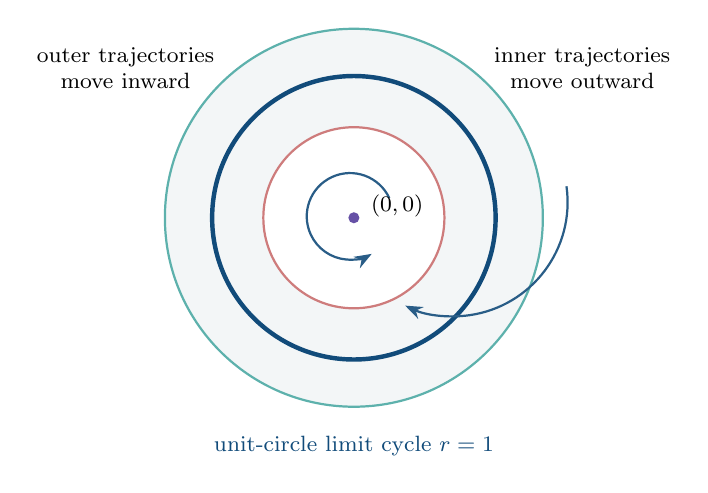
\begin{tikzpicture}
  \draw[fill=bmeglight, draw=bmegteal!70, thick] (0,0) circle (2.4);
  \draw[fill=white, draw=bmegred!70, thick] (0,0) circle (1.15);
  \draw[draw=bmegblue, ultra thick] (0,0) circle (1.8);
  \node[info, bmegblue] at (0,-2.9) {unit-circle limit cycle \(r=1\)};
  \draw[flow] (0.45,0.25) arc[start angle=25,end angle=300,radius=0.55];
  \draw[flow] (2.7,0.4) arc[start angle=8,end angle=-115,radius=1.45];
  \node[info] at (-2.9,1.9) {outer trajectories\\move inward};
  \node[info] at (2.9,1.9) {inner trajectories\\move outward};
  \fill[bmegpurple] (0,0) circle (2pt);
  \node[info] at (0.55,0.15) {\((0,0)\)};
\end{tikzpicture}
}
\end{center}

\subsection{State-space plots versus time plots}

The \MATLAB{} live script solves the model using \code{ode15s} and then makes two kinds of plots \cite{bmeg671MatlabNonlinearStability2025}:
\[
  t\mapsto w(t),z(t)
\]
and
\[
  w(t)\mapsto z(t).
\]
The first plot shows oscillation over time. The second plot is a phase portrait. A phase portrait starts at the initial condition \((w_0,z_0)\), not at \(t=0\) on an axis. The transcript spends time on this distinction because many beginners misread state-space plots as time plots.

Different initial conditions converge to the same unit circle, except the exact origin, which is a stationary point. In practice, exact unstable stationary points are fragile; a tiny perturbation moves away. That is another reminder that simulation initial conditions and biological initial conditions are not the same thing.

\subsection{Fox-rabbit dynamics are not the same kind of limit cycle}

The lecture then compares the classic prey-predator form:
\[
  \begin{aligned}
  \dot f &= arf-bf,\\
  \dot r &= cr-drf.
  \end{aligned}
\]
Depending on whether \(f\) denotes foxes and \(r\) rabbits, the signs are a matter of naming convention, but the structure is Lotka--Volterra-like: one state benefits from interaction, the other is harmed. The nonzero stationary point is
\[
  f^\ast=\frac{c}{d},\qquad r^\ast=\frac{b}{a}.
\]
Classical Lotka--Volterra systems can generate closed orbits whose amplitude depends on initial condition. That is not the same as an attracting limit cycle. A true attracting limit cycle pulls a range of initial conditions toward the same closed trajectory. This distinction matters in \QSP{} and disease modeling: repeated oscillation on a plot does not automatically mean robust biological rhythm.

\section{Parameter Ranges and Stability Maps}

\subsection{The symbolic workflow}

The stability live scripts show a useful \MATLAB{} pattern:
\begin{enumerate}[leftmargin=2em]
  \item declare symbolic variables with \code{syms};
  \item write the right-hand side \(f(\vect x,\vect\theta)\);
  \item solve \(f(\vect x,\vect\theta)=0\);
  \item compute \code{jacobian};
  \item substitute a stationary point and parameter values;
  \item compute eigenvalues with \code{eig};
  \item scan parameters and record whether \(\max\operatorname{Re}\lambda<0\).
\end{enumerate}
Mathematically this is simply the local stability theorem. Computationally it becomes a map from parameter space to qualitative behavior.

\subsection{Why a parameter scan is more than a plot}

For a model with uncertain parameters, a single stability conclusion can be misleading. Suppose a steady state is stable at the default parameter values. The next questions are:
\begin{center}
\begin{tabularx}{0.86\textwidth}{@{}XXX@{}}
stable for all plausible values? &
stable only in a narrow region? &
does a threshold boundary separate regimes?
\end{tabularx}
\end{center}
A contour plot of stable versus unstable regions is a qualitative uncertainty analysis. It does not replace parameter estimation, but it tells the modeler where inference and experiment matter most.

This point connects directly to model credibility. ICH M15 frames \MIDD{} evidence around the question of interest, model evaluation, and whether model outcomes are appropriate for a decision \cite{ichM15Midd2026}. A stability map is one kind of model evaluation: it shows whether a claimed qualitative behavior is robust to plausible parameter variation.

\section{Virus-Host Dynamics}

\subsection{The standard model}

The Sep 24 lecture uses a standard virus-host model:
\[
  \begin{aligned}
  \dot x &= \lambda-dx-\beta vx,\\
  \dot y &= \beta vx-ay,\\
  \dot v &= ky-wv.
  \end{aligned}
\]
Here \(x\) is uninfected target cells, \(y\) infected cells, and \(v\) free virus. The parameters have natural interpretations:
\begin{center}
\begin{tabularx}{0.9\textwidth}{@{}lll@{}}
\(\lambda\): target-cell production & \(d\): target-cell loss & \(\beta\): infection rate\\
\(a\): infected-cell loss & \(k\): virion production & \(w\): virion clearance
\end{tabularx}
\end{center}
The \MATLAB{} script uses symbolic algebra to solve stationary points, compute the Jacobian, and evaluate eigenvalues under numerical parameter values \cite{bmeg671MatlabNonlinearStability2025}.

\subsection{Disease-free and infected equilibria}

The disease-free equilibrium is
\[
  (x^\ast,y^\ast,v^\ast)=\left(\frac{\lambda}{d},0,0\right).
\]
The infection threshold is
\[
  \Rzero=\frac{\beta k\lambda}{adw}.
\]
When \(\Rzero>1\), an infected equilibrium exists:
\[
  x^\ast=\frac{aw}{\beta k},\qquad
  y^\ast=\frac{\lambda-dx^\ast}{a},\qquad
  v^\ast=\frac{k y^\ast}{w}.
\]
The algebra is less important than the interpretation. A virus establishes if infection of target cells and production of new virions overcome infected-cell death, virion clearance, and target-cell turnover. Again the course pattern reappears:
\[
  \text{stationary points}
  \longrightarrow
  \text{Jacobian}
  \longrightarrow
  \text{eigenvalues}
  \longrightarrow
  \text{biological regime}.
\]

\subsection{What the stability result does and does not say}

Local stability of an infected equilibrium says that small perturbations near that state return to it under the model. It does not say the model is clinically complete. Immune response, tissue compartments, drug treatment, latency, stochastic extinction, and measurement error may all matter for a real viral system. The stability result is still valuable because it tells us what the chosen three-state mechanism implies before we add more complexity.

\section{Dosing Workflows}

\subsection{Step inputs and piecewise simulation}

The vaccine model live script implements a piecewise dose:
\[
  \begin{aligned}
  \dot a &= -d_a a+u(t),\\
  \dot b &= \lambda-d_b b+eab.
  \end{aligned}
\]
The dose is not active for all time. The script therefore splits the simulation:
\[
  \begin{array}{ll}
  \text{before dose:} & u=0,\\
  \text{during dose:} & u=1,\\
  \text{after dose:} & u=0.
  \end{array}
\]
The final state of one segment becomes the initial condition of the next. In code, this is the pattern
\[
  \vect q_{\mathrm{next},0}=\vect x_{\mathrm{previous}}(\text{end},:).
\]
This is not a numerical trick. It is the mathematical statement that ODE trajectories are continuous across a dose interval unless the dose is modeled as an impulse.

\begin{center}
\resizebox{0.9\textwidth}{!}{%
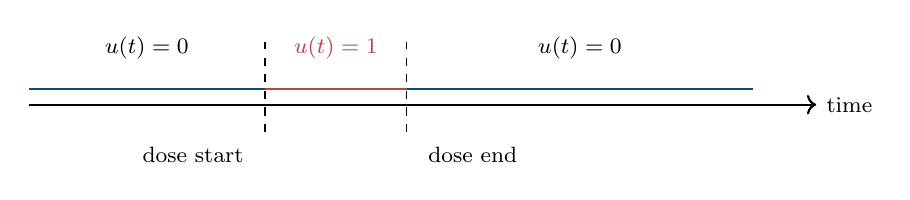
\begin{tikzpicture}
  \draw[->, thick] (0,0) -- (10,0) node[right,info]{time};
  \draw[thick, bmegblue] (0,0.2) -- (3.0,0.2);
  \draw[thick, bmegred] (3.0,0.2) -- (4.8,0.2);
  \draw[thick, bmegblue] (4.8,0.2) -- (9.2,0.2);
  \draw[dashed] (3.0,-0.35) -- (3.0,0.8);
  \draw[dashed] (4.8,-0.35) -- (4.8,0.8);
  \node[info] at (1.5,0.72) {\(u(t)=0\)};
  \node[info, bmegred] at (3.9,0.72) {\(u(t)=1\)};
  \node[info] at (7.0,0.72) {\(u(t)=0\)};
  \node[info, anchor=east] at (2.85,-0.64) {dose start};
  \node[info, anchor=west] at (4.95,-0.64) {dose end};
\end{tikzpicture}
}
\end{center}

\subsection{Why dose objects are useful in SimBiology}

\SimBio{} provides dose objects: target species, start time, interval, amount or rate, and repeat count. The Sep 24 transcript highlights a practical advantage: repeated dosing can be represented without manually splicing time intervals. For simple single scripts, manual segmentation is transparent. For repeated regimens, unit-checked dose objects are safer.

The choice is not ideological:
\begin{center}
\begin{tabularx}{0.88\textwidth}{@{}lX@{}}
\MATLAB{} equation script & maximum flexibility and transparent algebra\\
\SimBio{} model + dose object & unit checking, repeat dosing, sharing, and model management
\end{tabularx}
\end{center}
The mature workflow is to understand both and verify that they encode the same experiment.

\subsection{Parameter scans in dosing models}

The vaccine script scans the interaction parameter \(e\), which controls how antigen-like state \(a\) amplifies memory-like state \(b\). Qualitatively:
\[
  e \text{ small}: \text{weak amplification},
  \qquad
  e \text{ large}: \text{strong expansion}.
\]
But a large \(e\) may also make the model biologically implausible if \(b\) grows without saturation. That is a modeling clue. If a response variable should saturate, decline, or be resource limited, the equation may need a carrying capacity, immune contraction term, or feedback process.

\section{Exercises as Modeling Lessons}

\subsection{Stable and unstable stationary points}

For
\[
  \dot x=y(1-x),\qquad
  \dot y=x(1-y),
\]
the stationary points are \((0,0)\) and \((1,1)\). The Jacobian is
\[
  \J(x,y)=
  \begin{bmatrix}
  -y & 1-x\\
  1-y & -x
  \end{bmatrix}.
\]
At \((0,0)\),
\[
  \J=
  \begin{bmatrix}
  0&1\\
  1&0
  \end{bmatrix},
\]
with eigenvalues \(1\) and \(-1\), so the point is unstable. At \((1,1)\),
\[
  \J=
  \begin{bmatrix}
  -1&0\\
  0&-1
  \end{bmatrix},
\]
so the point is locally asymptotically stable.

The modeling lesson is that stationary points are not all equal. A model can contain both a repelling and attracting operating point, and a biological intervention can be interpreted as trying to move the system into the basin of attraction of the desired one.

\subsection{When a Lyapunov derivative changes sign}

If a proposed \(V\) yields
\[
  \dot V=x^3,
\]
then \(\dot V\) is positive when \(x>0\) and negative when \(x<0\). This does not prove stability or instability by itself. It proves only that the candidate \(V\) is not doing the job globally. The next move is to choose a different \(V\), restrict the domain if scientifically justified, or use another analysis.

\subsection{What failure of nonnegative invariance means}

If a state represents amount, concentration, population, or probability, negative values are not physically meaningful. If the nonnegative orthant is not positively invariant, then one of three things is usually true:
\begin{itemize}[leftmargin=2em]
  \item the model was intended only for a smaller domain;
  \item a missing nonlinear term or boundary mechanism should be added;
  \item the simulation or parameter values are being used outside their credible range.
\end{itemize}
This is not merely a mathematical flaw. It is a biological warning.

\section{A Practical Workflow for the Course Project}

\subsection{Before coding}

For a project model, write the following before opening \MATLAB{}:
\begin{itemize}[leftmargin=2em]
  \item state vector \(\vect x\), with units and biological meaning;
  \item input vector \(\vect u(t)\), including dose schedules or perturbations;
  \item output equation \(\vect y=g(\vect x,\vect\theta,t)\);
  \item parameter vector \(\vect\theta\), with plausible ranges;
  \item domain constraints such as \(\vect x\in\Rpos^n\);
  \item stationary points, if algebraically feasible;
  \item what data will be used for validation or fitting.
\end{itemize}

\subsection{While coding}

The live scripts imply a clean verification order:
\begin{enumerate}[leftmargin=2em]
  \item simulate a known or simple case;
  \item check signs and units;
  \item reproduce expected steady states;
  \item compare linear and nonlinear limits when a nonlinear model reduces to a linear one;
  \item plot both time courses and phase portraits;
  \item test multiple initial conditions;
  \item scan parameter ranges, not only one nominal value.
\end{enumerate}

\subsection{Before believing the result}

Ask:
\begin{center}
\fbox{\parbox{0.9\textwidth}{\centering Is the observed behavior a property of the model mechanism, a property of the chosen parameter values, a property of the initial condition, or a property of the numerical implementation?}}
\end{center}
This one sentence catches many errors. A stable equilibrium under one parameter set may disappear under another. A closed orbit may be a neutral Lotka--Volterra orbit rather than an attracting rhythm. A negative state may come from a structurally invalid model or from a solver step crossing a boundary. A beautiful \SimBio{} diagram may still encode the wrong rate law.

\section{Summary}

\subsection{One paragraph}

The September 8--26 BMEG 671 lectures move from writing compartmental equations to understanding dynamical behavior. \SimBio{} makes model grammar explicit: species, reactions, parameters, units, and doses. Linearization turns nonlinear systems into local linear approximations, making observability and controllability tests possible. Mass action, Michaelis--Menten, Hill functions, and logistic growth provide reusable kinetic building blocks. Stationary points organize long-run behavior; Jacobian eigenvalues classify local stability when the linear term is informative; Lyapunov functions handle cases where linearization is silent. Positive invariance protects biological domains such as nonnegative concentrations. Limit-cycle analysis distinguishes attracting oscillations from initial-condition-dependent loops. \MATLAB{} symbolic workflows and \SimBio{} dosing objects turn these ideas into reproducible modeling practice. The intellectual shift is from ``can I simulate this model?'' to ``what does this model necessarily imply, and can those implications support the question I care about?''

\subsection{The sentence to keep}

For every nonlinear biomedical model, ask:
\begin{center}
\fbox{\parbox{0.88\textwidth}{\centering What are the hidden states, what can I observe, what can I control, where are the equilibria, and which parts of state space are biologically allowed?}}
\end{center}
That sentence is the bridge from ODE syntax to scientific judgment.

\bibliographystyle{plain}
\bibliography{../refs/pharmacology}

\end{document}
